\documentclass[conference]{IEEEtran}

\usepackage[T1]{fontenc}
\usepackage[utf8]{inputenc}
\usepackage{cite}
\usepackage{amsmath,amssymb,amsfonts}
\usepackage{graphicx}
\usepackage{booktabs}
\usepackage{url}
\usepackage{hyperref}

\title{Base Paper: Crop Yield Prediction Using Machine Learning}

\author{%
\IEEEauthorblockN{Author Name}
\IEEEauthorblockA{Department Name\\
Institution Name\\
City, Country\\
email@domain.com}
}

\begin{document}

\maketitle

\begin{abstract}
This paper presents a baseline machine learning pipeline for crop yield prediction using tabular agricultural data. The workflow includes data preprocessing, model training, metric-based comparison, and deployment of the best model in a lightweight Flask web application. The dataset uses agronomic and environmental features such as location, crop type, weather variables, soil type, and fertilizer usage. Four regression models are evaluated: Random Forest Regressor, AdaBoost Regressor, Gradient Boosting Regressor, and Support Vector Regressor. In this project run, GradientBoostingRegressor achieved the strongest overall result with $R^2=0.946$, MAE $=0.231$, and RMSE $=0.277$. The paper provides a reproducible base structure that can be extended with real regional datasets and advanced feature sources.
\end{abstract}

\begin{IEEEkeywords}
Crop Yield Prediction, Machine Learning, Regression, Precision Agriculture, Flask
\end{IEEEkeywords}

\section{Introduction}
Reliable crop yield estimation supports farm planning, supply-chain decisions, and food-security analysis. Traditional methods often require high manual effort and may not adapt quickly to changing weather conditions. Machine learning can model nonlinear relationships among multiple agricultural variables and provide practical predictions.

This project implements an end-to-end crop-yield prediction system and exposes the selected model through a web application for interactive use.

\section{Objectives}
The objectives of this base study are:
\begin{itemize}
    \item Build a reproducible data-to-deployment machine learning pipeline.
    \item Compare multiple regression algorithms on the same feature space.
    \item Select the best-performing model using standard regression metrics.
    \item Provide a simple web interface for real-time inference.
\end{itemize}

\section{Dataset and Features}
The dataset contains the following columns:
\begin{itemize}
    \item Location: State, District
    \item Temporal and crop context: Crop\_Year, Season, Crop
    \item Production variables: Area, Production
    \item Weather variables: Rainfall, Temperature, Humidity
    \item Soil and input variables: Soil\_Type, Fertilizer\_Usage
    \item Target: Yield (tons/hectare)
\end{itemize}

If a dataset file is unavailable, the training pipeline can generate a synthetic dataset to preserve reproducibility of the workflow.

\section{Methodology}
\subsection{Preprocessing}
\begin{itemize}
    \item Missing-value imputation (median for numeric, most-frequent for categorical).
    \item One-hot encoding for categorical features.
    \item Standard scaling for numeric features.
    \item Train-test split with ratio 80:20.
\end{itemize}

\subsection{Models Evaluated}
\begin{itemize}
    \item RandomForestRegressor
    \item AdaBoostRegressor
    \item GradientBoostingRegressor
    \item Support Vector Regressor (RBF kernel)
\end{itemize}

\subsection{Evaluation Metrics}
\begin{itemize}
    \item Coefficient of determination ($R^2$)
    \item Mean Absolute Error (MAE)
    \item Root Mean Squared Error (RMSE)
\end{itemize}

\section{Results}
Table~\ref{tab:results} summarizes the model comparison from the current project output.

\begin{table}[htbp]
\caption{Regression Performance Comparison}
\label{tab:results}
\centering
\begin{tabular}{lccc}
\toprule
Model & $R^2$ & MAE & RMSE \\
\midrule
GradientBoostingRegressor & 0.946 & 0.231 & 0.277 \\
SVR & 0.939 & 0.212 & 0.296 \\
RandomForestRegressor & 0.919 & 0.280 & 0.341 \\
AdaBoostRegressor & 0.854 & 0.373 & 0.457 \\
\bottomrule
\end{tabular}
\end{table}

\begin{figure}[htbp]
\centerline{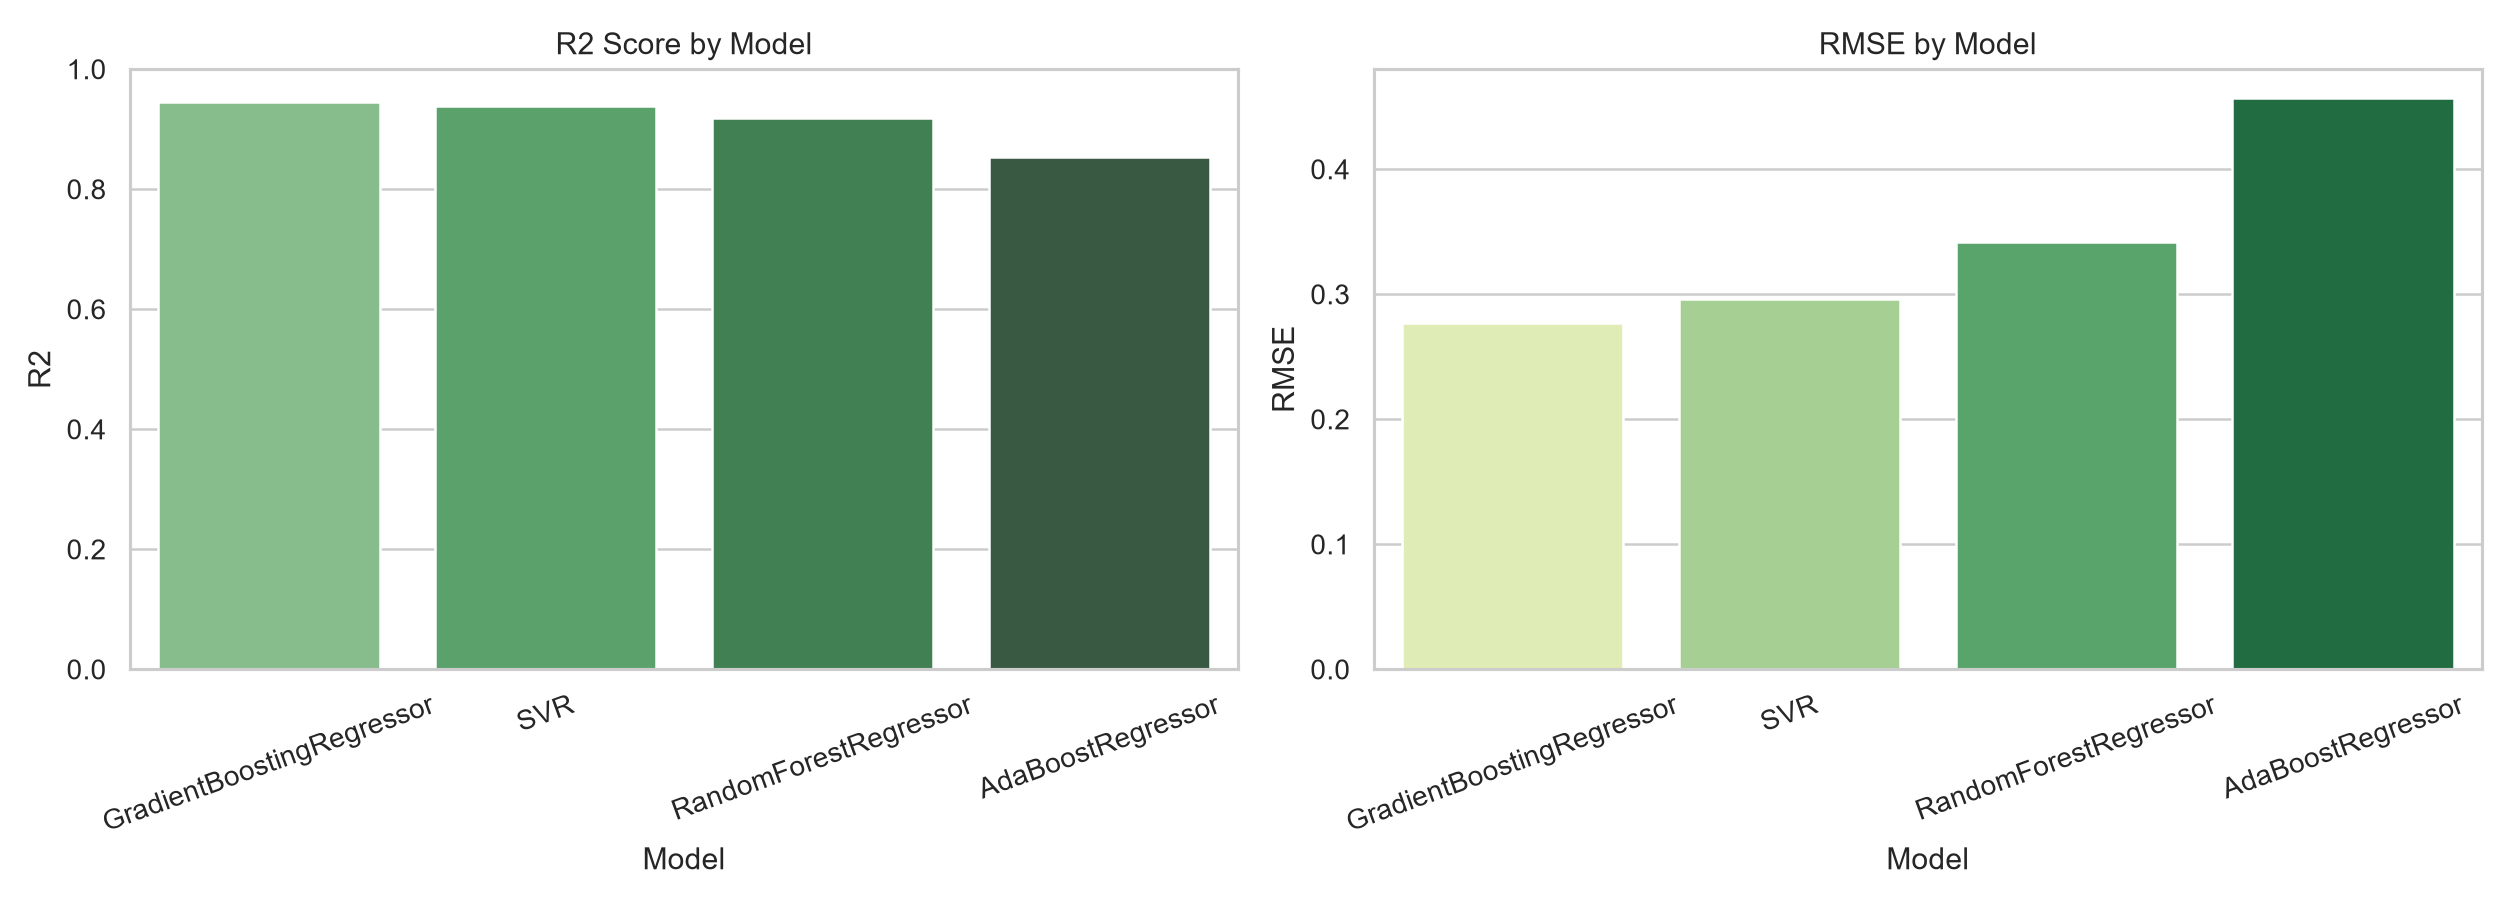
\includegraphics[width=0.48\textwidth]{static/model_comparison.png}}
\caption{Model comparison generated by the training pipeline.}
\label{fig:model-comparison}
\end{figure}

\begin{figure}[htbp]
\centerline{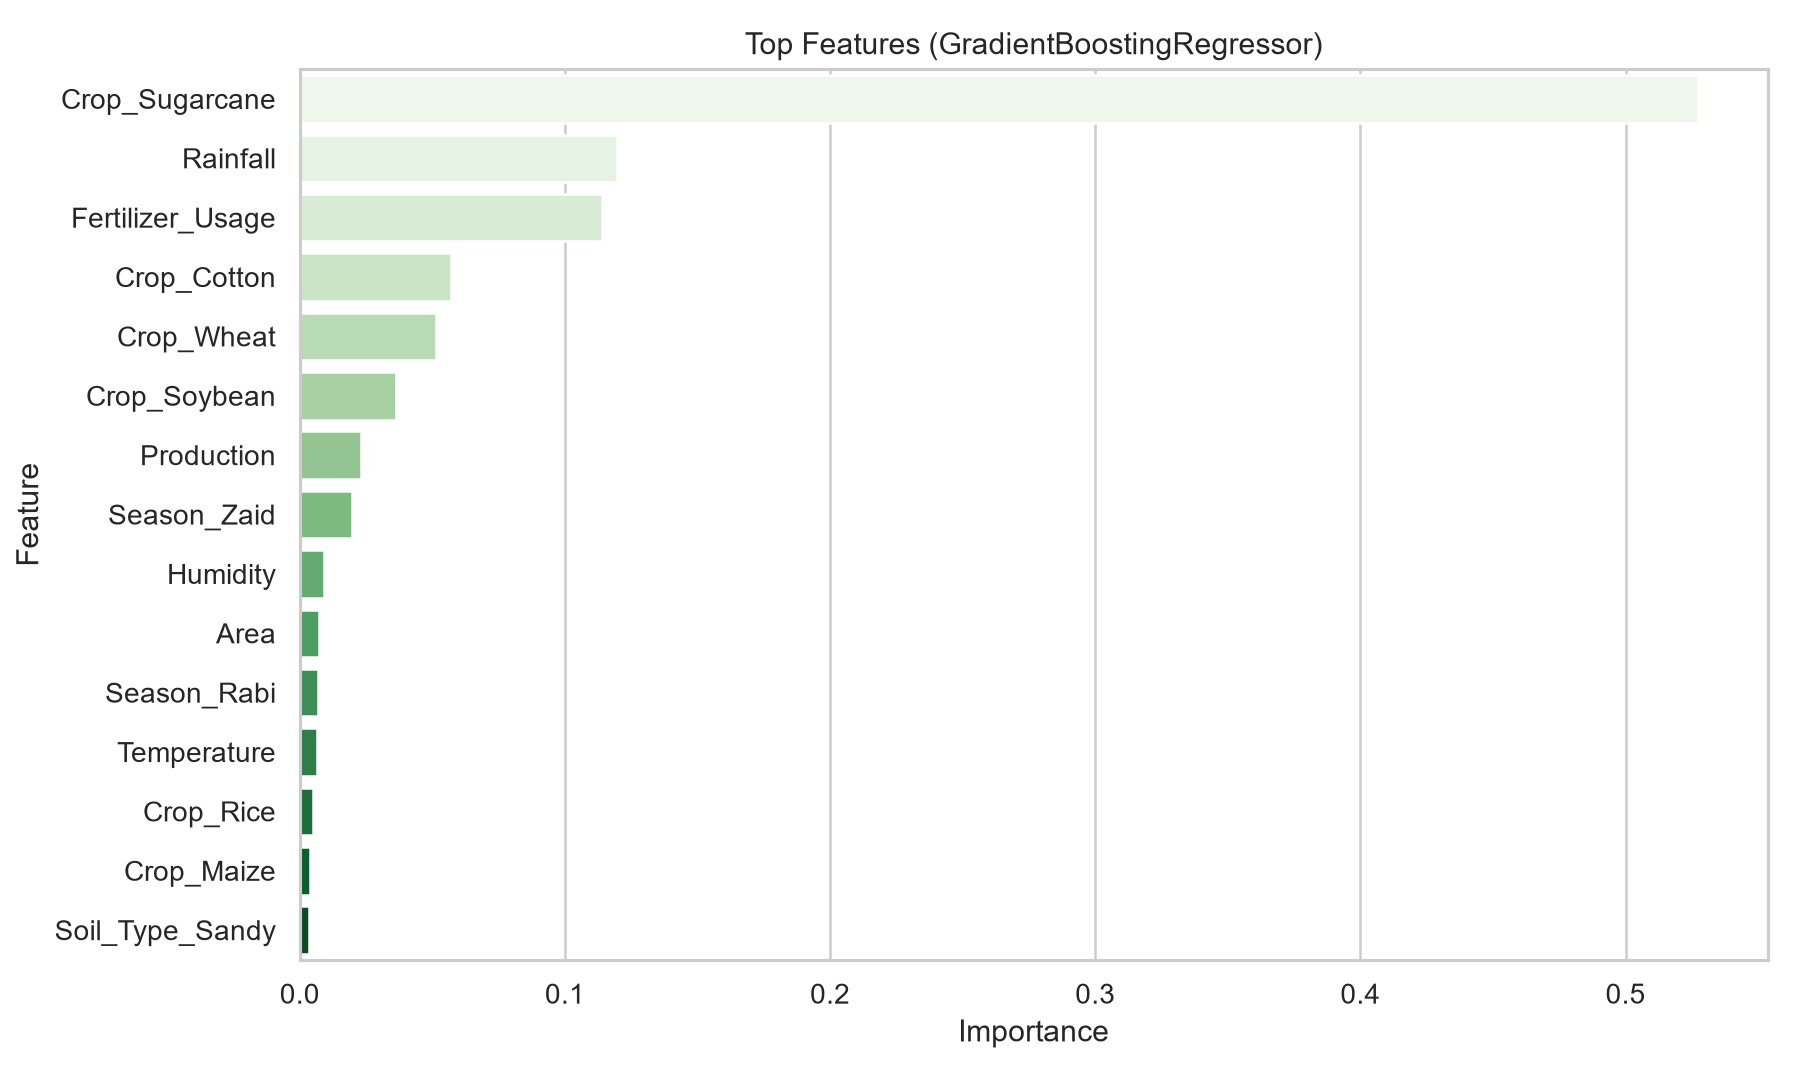
\includegraphics[width=0.48\textwidth]{static/feature_importance.png}}
\caption{Top feature importance values for the selected model.}
\label{fig:feature-importance}
\end{figure}

\section{Deployment}
The selected model is serialized to \texttt{model.pkl} and integrated into a Flask application for user-facing prediction. The application supports:
\begin{itemize}
    \item Input forms for all required features.
    \item Basic validation and error handling.
    \item User login/registration and prediction history.
\end{itemize}

\section{Conclusion}
This base paper demonstrates a complete and reproducible workflow for crop yield prediction using machine learning. GradientBoostingRegressor produced the best overall balance of accuracy and error metrics in this setup. The implementation can serve as a baseline for future work with larger real-world datasets, remote-sensing integration, and uncertainty-aware predictions.

\section{Future Work}
\begin{itemize}
    \item Train on district-level historical datasets with broader coverage.
    \item Integrate satellite-derived vegetation and climate indices.
    \item Add confidence intervals for risk-aware recommendations.
    \item Evaluate generalization across unseen regions and seasons.
\end{itemize}

\section*{Acknowledgment}
This work uses open-source tools from the Python data science ecosystem, including Scikit-learn and Flask \cite{sklearn,flask}.

\bibliographystyle{IEEEtran}
\bibliography{references}

\end{document}
